\documentclass[
   11pt,                        % Schriftgröße
   ngerman,                     % für Umlaute, Silbentrennung etc.
   a4paper,                     % Papierformat
   oneside,                     % einseitiges Dokument (muss zum drucken auf twoside geändert werden) 
   % openright,                 % Ungerade Seiten als Kapitelanfang (setzen wenn gedruckt werden soll)
   titlepage,                   % es wird eine Titelseite verwendet
   parskip=half,                % Abstand zwischen Absätzen (halbe Zeile)
   headings=normal,             % Größe der Überschriften verkleinern
   bibliography=totoc,          % Literaturverzeichnis im Inhaltsverzeichnis
   index=totoc,                 % Index im Inhaltsverzeichnis aufführen
   listof=totoc,                % Verzeichnisse im Inhaltsverzeichnis aufführen
   final,                       % Status des Dokuments (final/draft)
   numbers=noenddot,			% Kein Punkt hinter den Kapitelnummerierungen
   cleardoublepage=plain		% Plain sorgt dafür das Seitenzahlen noch auf leeren Seiten stehen
]{scrreprt}
%
%--Packages-------------------------------------------------------------------%
%
% Anpassung des Seitenlayouts 
\usepackage[
   automark, 					% Kapitelangaben in Kopfzeile automatisch erstellen
   headsepline, 				% Trennlinie unter Kopfzeile
   ilines 						% Trennlinie linksbündig ausrichten
]{scrlayer-scrpage}
%
% Anpassung an Landessprache 
%\usepackage[ngerman]{babel}
\usepackage[english]{babel}
%
% Encoding 
%\usepackage{fontspec}
%
% Euro-Zeichen etc.
\usepackage{textcomp}
%
% Subfigures
\usepackage{subfigure}
%
% Wrapfigures
\usepackage{wrapfig} 
%
% Mathe
\usepackage[intlimits]{amsmath}
\usepackage{amssymb}
\usepackage{empheq}
\usepackage{nicefrac}
\usepackage{upgreek}
\usepackage[
locale = US,
output-decimal-marker = {.}
]{siunitx}
\sisetup{locale=US, output-decimal-marker = {.}}
%
% Index
\usepackage{makeidx}
%
% Einfache Definition der Zeilenabsände und Seitenränder etc.
\usepackage{setspace}
\usepackage{geometry}
%
% Abkürzungsverzeichnis 
\usepackage[printonlyused]{acronym}
%
% zum Umfliegen von Bildern 
\usepackage{floatrow}
%
% einfachere Farbendefinition
\usepackage[usenames,dvipsnames]{xcolor}
%
% Programmcode 
\usepackage{listings}
%
% URL verlinken 
\usepackage{url}
%
% PDF-Optionen 
\usepackage[
   bookmarks,
   bookmarksopen=true,
   %diese Farbdefinitionen zeichnen Links im PDF farblich aus (zum drucken auskommentieren)
   colorlinks=true,
   linkcolor=blue, 			% einfache interne Verknüpfungen
   anchorcolor=black,			% Ankertext
   citecolor=blue, 			% Verweise auf Literaturverzeichnis im Text
   filecolor=magenta, 			% Verknüpfungen, die lokale Dateien öffnen
   menucolor=red, 				% Acrobat-Menüpunkte
   urlcolor=cyan,
   %
   plainpages=false, 			% zur korrekten Erstellung der Bookmarks
   pdfpagelabels, 				% zur korrekten Erstellung der Bookmarks
   hypertexnames=false, 		% zur korrekten Erstellung der Bookmarks
   linktocpage 				% Seitenzahlen anstatt Text im Inhaltsverzeichnis verlinken
]{hyperref}
%
% fortlaufendes Durchnummerieren der Fußnoten 
\usepackage{chngcntr}
%
% Tabellen 
\usepackage{tabularx}
\usepackage{multirow}
\usepackage{longtable}
\usepackage{colortbl}
\usepackage{array}
\usepackage{ragged2e}
\usepackage{lscape}
%
% bei der Definition eigener Befehle benötigt
\usepackage{ifthen}
%
% definiert u.a. die Befehle \todo und \listoftodos
\usepackage{todonotes}
%
% römische Zahlen
\usepackage{romannum}
%
% zum benutzen von toprule
\usepackage{booktabs}
%
% Rahmen
\usepackage{framed, color}
\usepackage[most]{tcolorbox}
%
% Biblioraphie
\usepackage{csquotes}
\usepackage[style=numeric, sorting=none, backend=biber]{biblatex}
%
% Tikz
\usepackage{color}
\usepackage{transparent}
\usepackage{pgfplots}
%
% Caption
\usepackage{caption}
%
% Platz hinter Komma
%\usepackage{ziffer}
%
% Tabellen farben
\usepackage{colortbl}
\usepackage{hhline}
%
% package pgf plots
\usepackage{pgfplots}
%
% bra-ket / dirac notation
\usepackage{braket}
%
%--Index----------------------------------------------------------------------%
%
\makeindex
%
%--Pfad zum Literaturverzeichnis----------------------------------------------%
%
\addbibresource{Verzeichnisse/Literatur.bib}
%
%--Meta-Informationen---------------------------------------------------------%
%
\newcommand{\titel}{NeNa}
\newcommand{\untertitel}{Untertitel}
\newcommand{\art}{Projektarbeit}
\newcommand{\fachgebiet}{Physik}
\newcommand{\autor}{Gabriel Sommer}
\newcommand{\studienbereich}{Physik}
\newcommand{\matrikelnr}{11912404}
\newcommand{\erstgutachter}{Andreas Grüneis}
\newcommand{\zweitgutachter}{Zweitprüfer}
\newcommand{\datum}{\today}
\newcommand{\ort}{Vienna}
%
%--Kopf- und Fußzeilen, Seitenränder etc--------------------------------------%
%
% Zeilenabstand 1,5 Zeilen 
\onehalfspacing
%
% Seitenränder
\setlength{\topskip}{\ht\strutbox} % behebt Warnung von geometry
\geometry{  paper=a4paper,
            inner=35mm,
            outer=30mm,
            top=25mm,
            bottom=25mm,
            footskip=10mm,
            includeheadfoot}
%
% Kopf- und Fußzeilen
\pagestyle{scrheadings}
%
% Schriftform der Kopfzeile
\renewcommand{\headfont}{\normalfont}
%
% Kopfzeile 
\ihead{\large{\textsc{\textit{\headmark}}}}
\chead{}
\ohead{}
%
% Höhe der Kopfzeile bei Chapter Anfang (ist riesig ohne diesen Kommentar)
\renewcommand*{\chapterheadstartvskip}{\vspace*{-\topskip}}
%
% Programmcode Style
\lstset{
   basicstyle=\ttfamily\footnotesize,
   identifierstyle=\color[rgb]{0,0,0},
   keywordstyle=\color[rgb]{0,0,1},
   stringstyle=\color[rgb]{0.56, 0.0, 1.0},
   commentstyle=\color[rgb]{0.18, 0.61, 0.33},
   columns=flexible,
   tabsize=2,
   extendedchars=true,
   showspaces=false,
   showstringspaces=false,
   numbers=left,
   numberstyle=\tiny,
   breaklines=true,
   backgroundcolor=\color[rgb]{0.9,0.9,0.9}}
%
\DeclareCaptionFont{white}{\color{white}}
\DeclareCaptionFormat{listing}{\colorbox[cmyk]{0.43, 0.35, 0.35, 0.01}{\parbox{\textwidth}{\hspace{0pt}#1#2#3}}}
\captionsetup[lstlisting]{
    format=listing,
    labelfont=white,
    textfont=white,
    singlelinecheck=false,
    margin=0pt,
    font={footnotesize},
}
%
% KOMA Optionen
\KOMAoptions{   
    headwidth=textwithmarginpar:0pt,    % Kopfzeile über den Text hinaus verbreitern
    headsepline=0.4pt}                  % Trennlinie unter Kopfzeile
%
% Fußzeile
\ifoot{}
\cfoot{\pagemark} % \pagemark in \ofoot schieben wenn gedruck werden soll
\ofoot{}
%
% erzeugt ein wenig mehr Platz hinter einem Punkt
\frenchspacing 
%
% Keine einzelnen Zeilen beim Anfang eines Abschnitts (Schusterjungen) 
\clubpenalty = 10000
%
% Keine einzelnen Zeilen am Ende eines Abschnitts (Hurenkinder)
\widowpenalty = 10000 \displaywidowpenalty = 10000
%
% Fußnoten fortlaufend durchnummerieren 
\counterwithout{footnote}{chapter}
%
% Floating-Umgebungen anpassen %
\renewcommand{\topfraction}{0.9}
\renewcommand{\bottomfraction}{0.8}
%
% Tiefe des Inhaltsverzeichniss
\setcounter{tocdepth}{1}
%
% captions of tables on top
\floatsetup[table]{capposition=top}
%
% pgf plot setup
\pgfplotsset{compat=newest}
\usetikzlibrary{plotmarks}
\usepgfplotslibrary{patchplots}
%
% damti auch im Druck alles immer die gleichen Abstände hat
\raggedbottom
%
%
%
%-----------------------------------------------------------------------------%
%
\begin{document}
%
%--Deckblatt------------------------------------------------------------------%
%
\thispagestyle{plain}
%
\begin{titlepage}
\begin{center}
%
\huge{\sffamily\textbf{\titel}}\\[3ex]
\LARGE{\sffamily\textbf{\untertitel}}\\[6ex]
\Large{\textbf{\art}}\\[1.5ex]
\Large{im Fachbereich \fachgebiet}\\[12ex]
%

\includegraphics[width=.7\linewidth]{Inhalt/Bilder/logo.png}\\[9ex]
%
\normalsize
%
\begin{table}[H]
\centering
\begin{tabular}{ll}
vorgelegt von:  & \quad \autor\\[1.2ex]
Studiengang: & \quad \studienbereich\\[1.2ex]
Matrikelnummer: & \quad \matrikelnr\\[1.2ex]
Erstprüfer:  & \quad \erstgutachter\\[1.2ex]
Zweitprüfer:  & \quad \zweitgutachter\\[16ex]
\end{tabular}
\end{table}
%
\datum
%
\end{center}
\end{titlepage}
%
%
%\myemptypage % setzen wenn zweiseitig gedruckt werden soll
%
%--Seitenzahl aus für Zusammenfassung-----------------------------------------%
%
\pagenumbering{gobble}
%
%---Abstract------------------------------------------------------------------%
%
\chapter*{Zusammenfassung}
%
Zugsamenfassung: Ziel, Methoden, Ergebnisse, Schlussfolgerungen
%
\clearpage{\thispagestyle{plain}\cleardoublepage}     
%
%--Seitenzahl groß Römisch für alle Verzeichnisse-----------------------------%
%
\pagenumbering{Roman}
%
%--Verzeichnisse--------------------------------------------------------------%
%
\tableofcontents                                      % Inhaltsverzeichnis
\listoffigures                                        % Abbildungsverzeichnis
\listoftables                                         % Tabellenverzeichnis
\lstlistoflistings                                    % Listings (Programmcode)
\addchap{Abkürzungsverzeichnis}
% 
\begin{acronym}[ABCDEFG]    % längstes Akronym in die eckige Klammer
%
\acro{API}{Application Programming Interface} 
\acro{LAMMPS}{Large-scale Atomic/Molecular Massively Parallel Simulator}
%
\end{acronym}
%          % Abkkürzungsverzeichnis
\addchap{Symbolverzeichnis}
% 
\begin{longtable}[l]{p{3cm}p{8cm}p{2cm}}
\setlength\tabcolsep{5pt}
Symbol & Bedeutung & Einheit \\
\hline
\endhead
\toprule
%
$B$ & magnetische Flussdichte & T \\
$D$ & Elektrische Flussdichte & A\,s\,m$^{-2}$ \\
%
\end{longtable}               % Symbolverzeichnis
%
\clearpage{\thispagestyle{plain}\cleardoublepage}   
%
%--arabische Seitenzahlen im Hauptteil ---------------------------------------%
%
\pagenumbering{arabic}
%
%--Inhalt---------------------------------------------------------------------%
%
\chapter{Einleitung}
\label{chap:Einleitung}
%
Einleitung: Wieso sollte diese Arbeit gelesen werden?
%
%
\chapter{Aufgabenstellung}
\label{chap:Aufgabenstellung}
%
We are here trying to calculate optical absorbtion spectra with vasp. The atomic configuration is a cavity inside a neon crystal that was proposed to be filled with either a single sodium atom or two sodiumm atoms (a sodium dimer). Now the first step was to find configurations of cavities, i.e. how many sodium neon atoms will be replaced by an inserted sodium atom and subsequntly by a sodium dimer. This substitution number will be denoted as $S$ in the following thesis. For these specific configurations the optical absorbtion spectra will be calculated and compared with the experiment.
%
%
\chapter{Theory}
\label{chap:Theory}
%
\section{Statistical Mechanics}
First we consider the system of the crystal of Neon Atoms as a canonical ensemble, this means it will be described under the assumption of an infinitely large heat bath by Boltzmann statistics. The probability distribution of members of the ensemble will then be 
\begin{align}
	p(\vec{\mathbf{q}},\vec{\mathbf{p}})=\frac{e^{-\beta H(\vec{\mathbf{q}},\vec{\mathbf{p}})}}{\int\cdots\int e^{-\beta H(\vec{\mathbf{q}},\vec{\mathbf{p}})}\mathrm{d}^{3N}\vec{\mathbf{q}}\mathrm{d}^{3N}\vec{\mathbf{p}}},
\end{align}
with $N$ being the number of particles.\\\\
Now an ensemble is to be understood as many fictional copies of the same system representing the states that a system will explore when propagating in time according to Hamilton's equation of motion. The ensemble distribution represents the relative number of times that an ergodic system will come by a given state after an infinite amount of time has passed. Now for a crystal in principle this still holds. At low temperatures though the phase space that is being explored can be abstracted in such cases. The reason is that the system will for a given time usually explore only nearby points in the phase space. This is the crystal configuration but allowing for dynamics such as lattice vibrations and thermal movement of the atoms with respect to their lattice site. So for a given initial point in phase space the system will mostly explore its proximity until it probabilistically jumps to another volume of phase space whose proximity then will be explored for some further time. Now this means the systems lattice configuration has changed which at low but non zero temperature should be reasonable. 
We now consider these volumes of phase space (being approximately confined regions, i.e. configurations of e.g. a crystalline structure) to be discrete states that the system can be in. So our canonical distribution now is a discrete one, each state representing such a configuration volume. What's left is to figure out what state of the still continuously possible states inside will be used to represent each configuration. We in this work will use the state $(\vec{\mathbf{q}}_{0i},\vec{\mathbf{p}}_{0i})$ that locally minimizes $H(\vec{\mathbf{q}},\vec{\mathbf{p}})$. Such a minimum can be found by employing a relaxation calculation in LAMMPS. The Boltzmann distribution now follows to be:
\begin{align}
	p(\vec{\mathbf{q}}_{0i},\vec{\mathbf{p}}_{0i})=\frac{e^{-\beta H(\vec{\mathbf{q}}_{0i},\vec{\mathbf{p}}_{0i})}}{\sum_{n} e^{-\beta H(\vec{\mathbf{q}}_{0n},\vec{\mathbf{p}}_{0n})}}.
\end{align}

grand canonical ensemble with two chemical components

sub term of grand canonical ensemble with only ne1 and ne2
\section{Relaxation in LAMMPS}
relaxation theory form lammps 
described in Bitzek, Koskinen, Gahler, Moseler, Gumbsch, Phys Rev Lett, 97, 170201 (2006)
 
\section{Simulated Annealing}
Molecular Dynamics simulation

Hopefully explanation for cohesive energy


%
%

\chapter{Finding Minima of Neon Replacements}
\label{chap:Erstes Kapitel}
\section{Pair Potential Interaction}
\subsection{\ac{HF} equations}
We start with the pair potentials of Ne-Ne, Ne-Na and Na-Na to mimic the interaction of long distance van der Vaals + short distance repulsion forces. The pair potentials have been calculated using a \ac{HF} self consistent field cycle with \ac{MP2} by varying the atom distance. Now selfconsistently solving the equations:\\
\begin{align}
	\left[-\frac{\hbar^2}{2m}\vec{\nabla}^2-\frac{Ze^2}{4\pi\varepsilon_0}-\frac{e^2}{4\varepsilon_0}\sum_{\nu,\sigma}^{(\mu\sigma)\neq(\nu\sigma)}\iiint_{\mathbb{R}^3}\frac{\varphi_{\nu\sigma'}(\tilde{\vec{r}})}{\|\vec{r}-\tilde{\vec{r}}\|}\mathrm{d}^3\tilde{\vec{r}}-\hat{A}_{\mu\sigma}(\vec{r})\right]\varphi_{\mu\sigma}(\vec{r})=\varepsilon_{\mu\sigma}\varphi_{\mu\sigma}(\vec{r}),
\end{align}
with $\hat{A}_{\mu\sigma}$ being the exchange correlation term leads to the eigenenergies $\varepsilon_{\mu\sigma}$. Since \ac{HF} 
minimizes a slater determinant, the energies correspond to the factors of the slater product state, meaning the systems energy is the sum of the energy of the single electrons. From that, to get the actual energy of the whole system, one needs to remove inter-electron repulsion and exchange correlation from the sum of all eigenenergies $\varepsilon_{\mu\sigma}$:
\begin{align}
	E_{HF}^0 = \sum_{\mu,\sigma}\varepsilon_{\mu\sigma}-\frac{1}{2}\sum_{\substack{\mu,\nu\\\sigma,\sigma'}}^{(\mu\sigma\neq\nu\sigma)}\left[C_{\mu\sigma}^{\nu\sigma'}-A_{\mu\sigma}^{\nu\sigma}\delta_{\sigma\sigma'}\right]
\end{align}
with $C_{\mu\sigma}^{\nu\sigma'},A_{\mu\sigma}^{\nu\sigma}$ being defined as:
\begin{align}
	C_{\mu \sigma}^{v \sigma^{\prime}}&=\frac{e^2}{4 \pi \varepsilon_0} \iint  \frac{\left|\varphi_{\mu \sigma}(r)\right|^2\left|\varphi_{v \sigma^{\prime}}\left(r^{\prime}\right)\right|^2}{\left|r-r^{\prime}\right|}\mathrm{~d}^3 r \mathrm{~d}^3 r^{\prime},
	\\
	A_{\mu \sigma}^{v \sigma}&=\frac{e^2}{4 \pi \varepsilon_0} \iint \frac{\varphi_{\mu \sigma}^*(r) \varphi_{v \sigma}^*\left(r^{\prime}\right) \varphi_{\mu \sigma}\left(r^{\prime}\right) \varphi_{v \sigma}(r)}{\left|r-r^{\prime}\right|} \mathrm{~d}^3 r \mathrm{~d}^3 r^{\prime}.
\end{align}
Since solving the \ac{HF} equations in real space is too costly one restricts the variations to coefficients of a superposition of fixed basis vectors. These lead to the Roothaan-Hall equations, which are a discrete Matrix representation of the \ac{HF} equations:
\begin{align}
	\mathbf{F C}=\mathbf{S C} \epsilon,
	\label{eq:roothaan}
\end{align} 

with $\epsilon$ being a diagonal matrix of single particle energies on the diagonal, $\mathbf{S}$ the basis overlap matrix, $\mathbf{C}$ the coefficient matrix and finally $\mathbf{F}$ the Fock operator.
\subsection{Møller-Plesset Perturbation}
Møller-Plesset Perturbation theory extends the idea of \ac{HF}. We consider the actual true Hamiltonian  $\hat{H}$ in the same basis as \ref{eq:roothaan} and define the difference to the Fock operator to be a relatively small perturbation:
\begin{align}
	\hat{H}= \hat{F} + \underbrace{\left(\hat{H}-\hat{F}\right)}_{\hat{V}_{pert}}.
\end{align} THe $0$-th order Term is just the sum of the eigenvalues $\varepsilon_i$ of the Fock Problem.
Now the $1$st order terms of the perturbation are
\begin{align}
	E^{(1)}&=\bra{\Psi_{HF}}\left(\hat{H}-\hat{F}\right)\ket{\Psi_{HF}}=\\
	&=-\frac{1}{2}\sum_{\mu\nu}\left[\bra{\varphi_{\mu}\varphi_{\nu}}\hat{V}^{(2)}(\hat{\vec{r}}_\mu,\hat{\vec{r}}_\nu)\ket{\varphi_{\mu}\varphi_{\nu}}-\bra{\varphi_{\mu}\varphi_{\nu}}\hat{V}^{(2)}(\hat{\vec{r}}_\mu,\hat{\vec{r}}_\nu)\ket{\varphi_{\nu}\varphi_{\mu}}\right].
\end{align} 
which is exactly the mean-field and the exchange correlation term in the \ac{HF} Ansatz, so to go beyond \ac{HF} we need to consider \ac{MP2}:
\begin{align}
	E^{(2)}=\sum_{\substack{N<a<b \\ \mu<\nu \leq N}} \frac{\left|\bra{\psi_0}\hat{V}^{(2)}(\hat{\vec{r}}_\mu,\hat{\vec{r}}_\nu)\ket{\psi_{\mu\nu}^{a b}}\right|^ 2}{\left(\varepsilon_a+\varepsilon_b\right)-\left(\varepsilon_\mu+\varepsilon_\nu\right)} .
\end{align} where $\ket{\psi_{\mu\nu}^{a b}}$ is an excited Slater determinant, where single orbitals $\mu, \nu$ are removed and replaced by single orbitals $a,b$ in the slater determinant. $\varepsilon_i$ are eigenvalues of the slater single particle factors of the \ac{HF} problem.
\subsection{\ac{BSSE}}
Now the the superpositions of a fixed basis leads to the \ac{BSSE}. These errors are being corrected for by using 'ghost calculations', essentially the same calculation with one atom being removed (i.e. the extended two atom centered basis stays the same). This means the basis will have access to the second electron states, but the nucleus and additional electrons are not accounted for. These 'ghost energies' will then subsequently be removed from the \ac{HF}
approximation to correct for the \ac{BSSE}.
This is know as the counterpoise‐corrected interaction energy formula or Boys–Bernardi method: %TODO citation %TODO fix formula
\begin{align}
	E_{\text {int}}^{\text {CP}}(R)=E_{A B}(R)-E_A^{\text {ghost}}(R)-E_B^{\text {ghost}}(R).
\end{align}
Here $E_{A B}(R)$ is the energy after \ac{MP2} and $E_A^{\text {ghost}}(R),E_B^{\text {ghost}}(R)$ refer to the same calculation results, just with one atom removed completely.
\subsection{Interpolation}

\begin{figure}[h!]
	\centering
	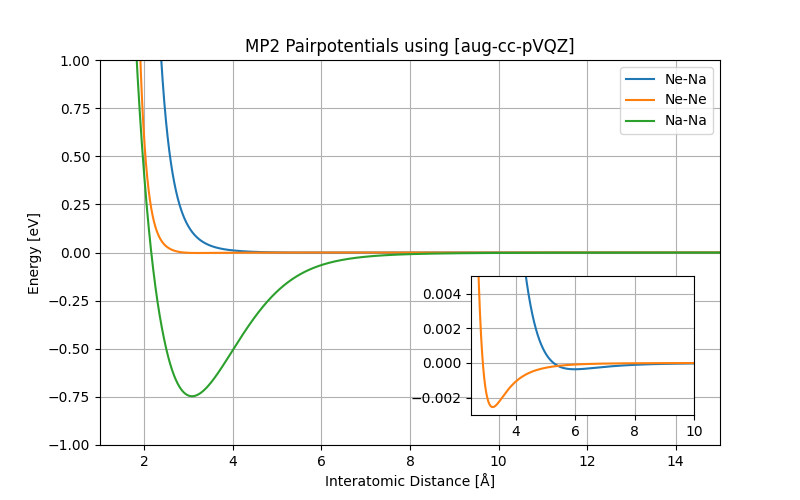
\includegraphics[scale = 0.7]{Inhalt/Bilder/pairpotential.png}
	\caption{Plots of interpolations of pair potentials of Ne-Ne, Na-Na, Ne-Na calculated with Moeller Plesset 2 perturabtion theory.}
	\label{fig:pairpotential}
\end{figure}
%TODO Noltig source
-explain exact interpolation\\
-paper citation where brute force plot shows up as well\\
-which basis is being used in the roothaan equations \\
-explain setup of calculation with ball being carved out\\
-maybe here explain the nearest neighbours\\
lammps gets linear interpolation\\
-since plot is in priniple linearly interpolated this is the exact pair interactins that lammps will read
\section{Geometric LAMMPS Setup}
%%%%%%%%%%%%%%%%%%%%%%%%%%%%%%%%%%%%%TODO%%%%%%%%%%%%%%%%%%%%%%%%%%%
The simulation models a finite spherical cluster of atoms extracted from a bulk face-centered cubic lattice. To balance computational efficiency with physical realism, the system is partitioned into two concentric spherical regions defined in units of the lattice constant. The inner spherical region, with radius $n_{inner}$ contains atoms that are free to move and evolve dynamically. This region represents the core of the cluster where physical process and in this case the energy minimization via a relaxation calculation of \ac{LAMMPS} takes place.

Sourrounding this core is an immobilized shell with thickness $n_{outer}$
Atoms within this outer shell are constrained by setting their forces to zero, effectively fixing them in space. This fixed shell act as a rigid boundary that suppresses surface effects and mimics the presence of a an extended bulk lattice, thereby reducing finite size artifact in the dynamics of the inner region.

Consequently the total cluster is confined within a spherical domain of radius $R_{tot}=(n_{inner}+n_{outer})\cdot a$ with $a$ being the lattice constant of the pure neon \ac{fcc} lattice. 

Technically the simulation is defined as a cubic volume large enough to contain the entire spherical cluster, with half-length at least $R_{tot}$.
For the relaxation mechanics atomic positions are set according to \ref{fig:lammpssetup} on a perfect \ac{fcc} lattice no matter their role (sodium defect, fixed neon, dynamic neon) as long as they are inside the cutoff radius $R_{tot}$.
%TODO is it really ? check, cite
This approach is commonly employed in molecular dynamics studies to simulate nanoparticles or finite clusters embedded in bulk-like surroundings.
%%%%%%%%%%%%%%%%%%%%%%%%%%%%%%%%%%%TODO%%%%%%%%%%%%%%%%%%%%%%%%%%%%%%%%%%%
\begin{figure}[h!]
	\centering
	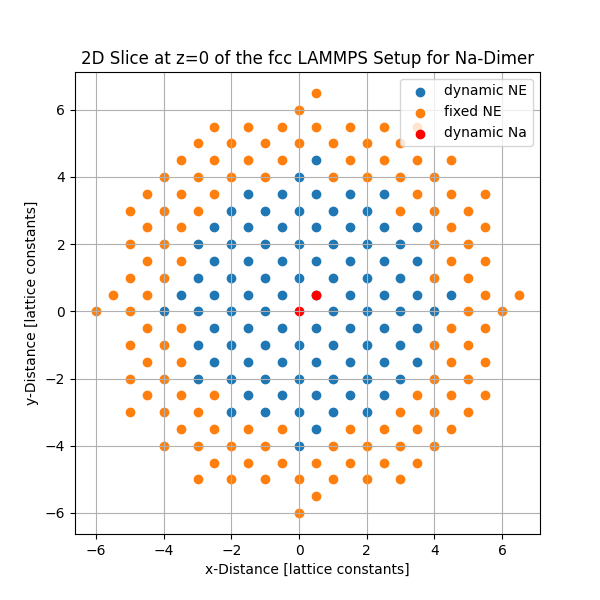
\includegraphics[scale=0.45]{Inhalt/Bilder/lammps_dimer_setup.png}
	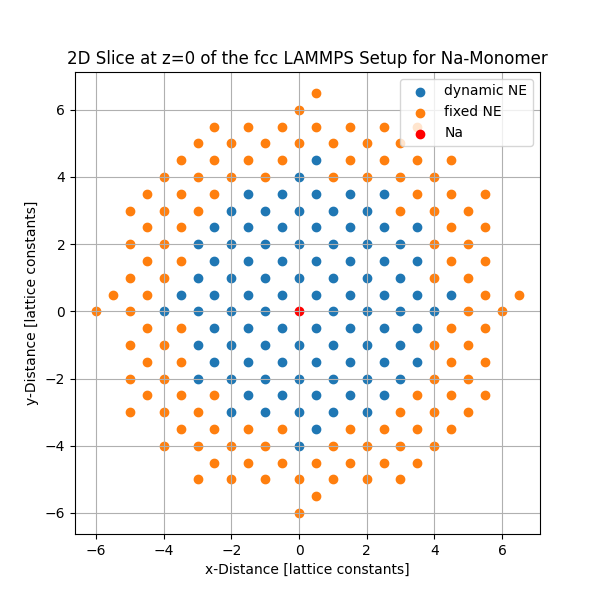
\includegraphics[scale=0.45]{Inhalt/Bilder/lammps_mono_setup.png}
	\caption{Initial setup for the \ac{LAMMPS} relaxation. Only the inner blue sphere is allowed to relax, forces on the orange atom positions are overridden to 0.}
	\label{fig:lammpssetup}
\end{figure}\\%TODO split figure into subfigures with exra captions
The centered red dots in \ref{fig:lammpssetup} represent sodium atoms. They represent the initial pre-relaxation positions of sodium inside the dynamic inner sphere. These initial positions are the same for every relaxation step of the simulated annealing. Note that the minimum energy of the pair-potential in \ref{fig:pairpotential} is roughly at $3\text{.}1\si{\angstrom}$ which is the nearest neighbor distance in the neon \ac{fcc} lattice. With $a = 4\text{.}4637\si{\angstrom}$: 
%TODO fix unit separator to a dot, onyl comma works for now
\begin{gather}
	\vec{a}_1=\begin{bmatrix}a\\0\end{bmatrix} \qquad \vec{a}_2=\begin{bmatrix}0\\a\end{bmatrix}\\
	\Rightarrow \|\frac{1}{2}\left(\vec{a}_1+\vec{a}_2\right)\|=\frac{1}{\sqrt{2}}\cdot a = 3\text{.}1563\si{\angstrom}.
\end{gather}  We therefore put the second sodium atom in the dimer calculations at the nearest neighbor lattice site and Set th initial removal $S$ to $S=2$. 
\section{Sodium Monomer}
Now the annealing was done as described in the chapters before for a single sodium atom at the center. Since the known energetically minimal configurations for every $S$ and it's corresponding energy was known due to a brute force calculation, this calculation serves as a benchmark for the annealing algorithm. The brute force minimal energies for the vacancies are shown in \ref{fig:simulatedannealingsodium} on the right axis. The left axis shows the relative counts (with respec to the total counts) of one annealing sweep consisting of itself 1000 random removals of neon atoms from the state vector. This annealed approach quickly converges to a statistical distribution shown in the same figure \ref{fig:simulatedannealingsodium} on the left $y$-axis. The pattern surfaces quickly after about 50 sweeps, the total amount of sweeps for the plot were 736. The true local minima at $S=10$ and $S=13$ could be picked up upon quite sharply. At $S=8$ the annealing algorithm seems to pick up on the notch, that is not quite an actual minima but could look like a local minima if approached from many directions in the high dimensional phase space.\\  

-explain how plot is created with sweeps\\
-more complicated symmetries\\
-compare figures\\
-calculation for dimer\\
-discuss noteworthy structure (e.g. inner shell carved out)\\
-citation of paper that has the same plot
Now first by brute force search we know the minima for a single sodium atom.

%\begin{figure}[h!]
%	\centering
%	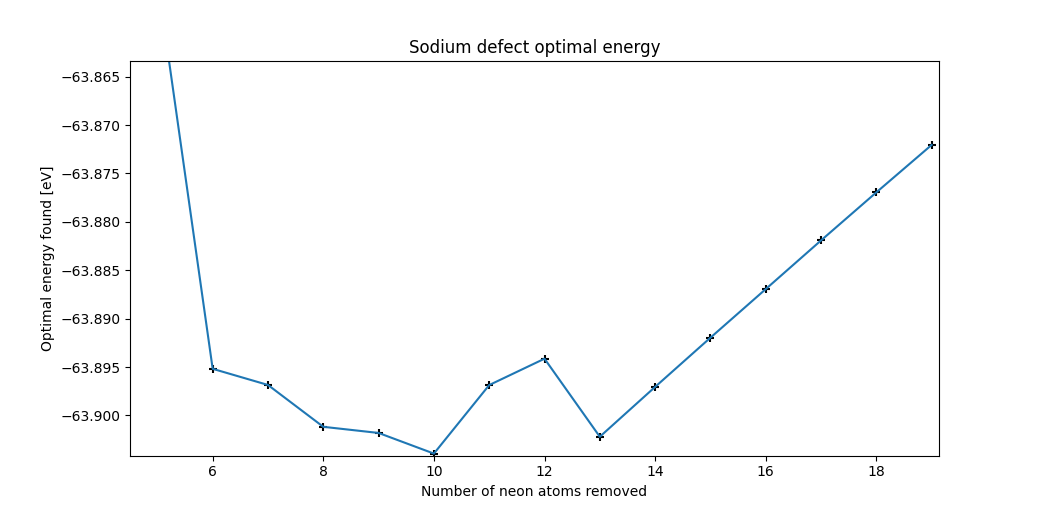
\includegraphics[scale=0.5]{./Inhalt/Bilder/optimal_defect_brute_force.png}
%	\caption{Brute force for single sodium atom}
%	\label{fig:bruteforcesodium}
%\end{figure}

\begin{figure}[h!]
	\centering
	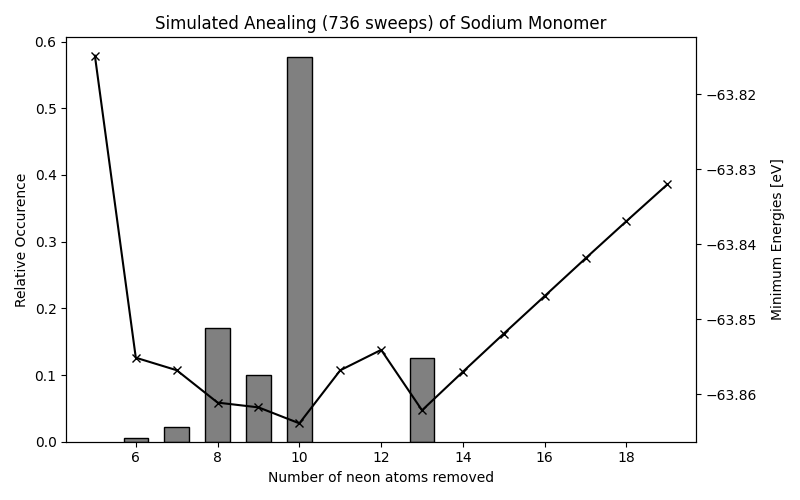
\includegraphics[scale=0.5]{./Inhalt/Bilder/optimal_defect_simulated_annealing.png}
	\caption{Simulated Annealing for single sodium atom inserted, compared to a brute force minima search for a fixed number of removed atoms S.}
	\label{fig:simulatedannealingsodium}
\end{figure}  



-brute force lexiciraphically sorting algorithm here

\section{Sodium Dimer}
Since \ref{fig:simulatedannealingsodium} shows the simulated annealing algorithm accurately picks up on the location of the minima (albeit with no quantitative measure and misleading local minima being blown out of proportion (See $S=8$)) we try the same approach for the sodium dimer. Here the energetically optimal $S$ replacement will expectantly going to exceed the number of available sites as in the monomer calculation (i.e. up to second nearest neighbor). The sweeps and their random removal of neon atoms now act upon an extended state vector containing every lattice site up to the 3rd nearest neighbor. This is also the very reason a brute force approach is unfeasible, since the volume of phase space to be explored grows quickly. Considering the octahedral symmetry $O_h$ of the host, which the defect cannot possibly exceed and roughly estimating one minimization run to take about $20\si{\second}$, we get $\frac{2^{42}}{48}\cdot20s\approx10^{12}s$ which exceeds realistic rescources for a brute force attack. This is the reason the statistical approach was chosen in the first place. 

- symmetry\\
-heuristically take the maxima of these plots \\
-give structures\\
-discuss structures (inner shell carved out)\\

\begin{figure}[h!]
	\centering
	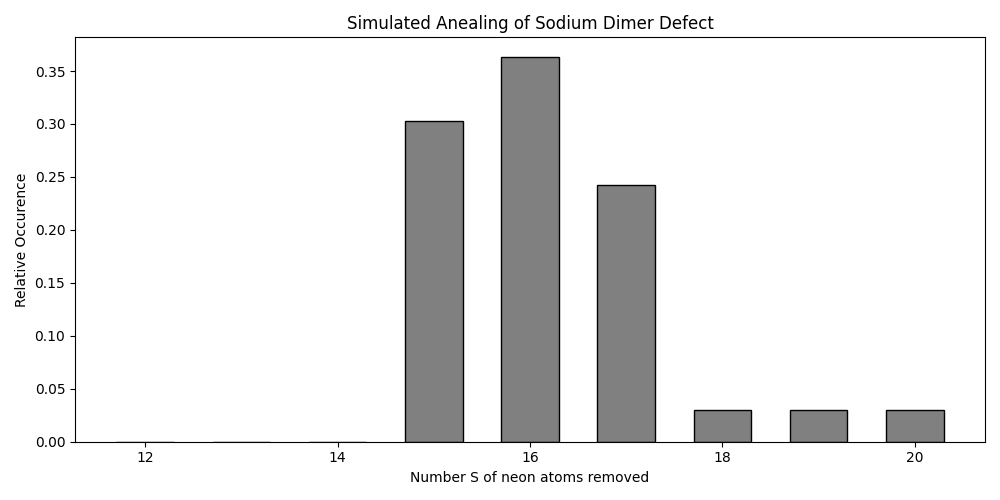
\includegraphics[scale = 0.5]{Inhalt/Bilder/optimaldimer.png}
	\caption{Simulated annealing results and their relative occurrence after x sweeps}
	\label{fig:simulatedannealingsodiumdimer}
\end{figure}

\chapter{DFT optical spectra results}
\label{chap:Zweites Kapitel}
%
Zweites Kapitel
%
%
\chapter{Conclusion}
Unfortunately no confidence or error can be estimated since the approach was purley heuristcal. Optical spectrum does not depend much on replacements and precise structure.




%
\chapter{Ausblick}
\label{chap:Ausblick}
%
Ausblick
%
%
\clearpage{\thispagestyle{plain}\cleardoublepage}   
%
%--kleine römische Seitenzahlen für den Rest----------------------------------%
%
\pagenumbering{roman}
%
%--Literaturverzeichnis-------------------------------------------------------%
%
\printbibliography
%
%--Anhang---------------------------------------------------------------------%
%
\appendix
%
\chapter{Anhang}
\label{chap:Anhang}
%
\section{Inhalt des beigefügten Datenträgers}
\label{sec:Inhalt des beigefügten Datenträgers}
%
\newcommand{\itemCustom}[1]{\item[] \includegraphics[height=\baselineskip]{Inhalt/Bilder/Icons/#1}~}
\newcommand{\itemPDF}{\itemCustom{application-pdf}}
\newcommand{\itemFolder}{\itemCustom{folder-yellow}}
\newcommand{\itemDatei}{\itemCustom{Datei}}
\newcommand{\itemDisc}{\itemCustom{media-optical}\texttt}
%
\begin{itemize}
	\itemDisc \texttt{Datenträger}
	\begin{itemize}
		\itemFolder \texttt{A}
		\begin{itemize}
			\itemFolder \texttt{a}
			\itemFolder \texttt{b}
			\itemFolder \texttt{c}
		\end{itemize}
	\end{itemize}
	\begin{itemize}
		\itemFolder \texttt{B}
		\begin{itemize}
			\itemFolder \texttt{a}
			\itemFolder \texttt{b}
		\end{itemize}
	\end{itemize}
	\begin{itemize}
		\itemPDF \texttt{A}
	\end{itemize}
\end{itemize}
%
\let\itemCustom\undefined
\let\itemPDF\undefined
\let\itemFolder\undefined
\let\itemDisc\undefined
%
%
%--Selbständigkeitserklärung--------------------------------------------------%
%
\chapter*{Eidesstattliche Erklärung}
%
Ich, \autor, versichere hiermit, dass ich die vorliegende Arbeit
selbstständig verfasst und keine anderen als die angegebenen Quellen und Hilfsmittel benutzt habe, wobei ich alle wörtlichen und sinngemäßen Zitate als solche gekennzeichnet habe.\par
%
Diese Arbeit wurde bisher in gleicher oder ähnlicher Form keiner anderen Prüfungsbehörde vorgelegt und auch nicht veröffentlicht.\\[5ex]
%
\ort, den \datum\\[5ex]
%
\rule[-0.2cm]{5cm}{0.5pt}\\
%
\textsc{\autor} 

\chapter*{Declaration of Authorship}
%
I, \autor, hereby declare that I have written the present thesis independently and have used no sources or aids other than those explicitly stated. All direct quotations and all paraphrased ideas have been clearly marked as such.\par
%
This work has not been submitted, either in the same or a substantially similar form, to any other examination board, nor has it been published elsewhere.\\[5ex]
%
\ort, \datum\\[5ex]
%
\rule[-0.2cm]{5cm}{0.5pt}\\
%
\textsc{\autor}
%
%-----------------------------------------------------------------------------%
%
\end{document}
%